% CS615A Aspects of System Administration
% Author: Jan Schaumann <jschauma@netmeister.org>
% $Id: slides.tex,v 1.12 2006/02/12 23:15:03 jschauma Exp $

\special{! TeXDict begin /landplus90{true}store end }

\documentclass[xga]{xdvislides}
\usepackage[landscape]{geometry}
\usepackage{graphics}
\usepackage{graphicx}
\usepackage{colordvi}
\usepackage{tabularx}
\usepackage{multirow}

\newcommand{\gargantuan}{\fontsize{100}{105}\selectfont}

\begin{document}
\setfontphv

%%% Headers and footers
\lhead{\slidetitle}                               % default:\lhead{\slidetitle}
\chead{CS615 - Aspects of System Administration}% default:\chead{\relax}
\rhead{Slide \thepage}                       % default:\rhead{\sectiontitle}
\lfoot{\Gray{Software Packaging, Multiuser Fundamentals, Ethics}}% default:\lfoot{\slideauthor}
\cfoot{\relax}                               % default:\cfoot{\relax}
\rfoot{\Gray{\today}}

\vspace*{\fill}
\begin{center}
	\Hugesize
		CS615 - Aspects of System Administration\\ [1em]
		Software Packaging, Multiuser Fundamentals, Ethics\\ [1em]
	\hspace*{5mm}\blueline\\ [1em]
	\Normalsize
		Department of Computer Science\\
		Stevens Institute of Technology\\
		Jan Schaumann\\
		\verb+jschauma@stevens.edu+\\
		\verb+http://www.cs.stevens.edu/~jschauma/615/+
\end{center}
\vspace*{\fill}

\subsection{Why use a Package Management System?}
\begin{verbatim}
$ aws ec2 run-instances --image-id ami-6de0dd04 # Ubuntu
$ aws ec2 run-instances --image-id ami-3b361952 # Fedora
\end{verbatim}

\subsection{Why use a Package Management System?}
\begin{itemize}
	\item easy and scalable installation of software
	\item automatic resolution of software dependencies
	\item package and file inventory \\
\begin{verbatim}
linux-lab$ dpkg -l
[...]
linux-lab$ dpkg -L tcpdump
[...]
linux-lab$ dpkg-query -S /usr/lib/libsqlite.so.0.8.6 /usr/bin/sqlite3
[...]

\end{verbatim}
\end{itemize}

\subsection{Why use a Package Management System?}
\begin{itemize}
	\item easy and scalable installation of software
	\item automatic resolution of software dependencies
	\item package and file inventory
	\item integration into OS
		\begin{itemize}
			\item OS-specific defaults / config files
			\item creation of service accounts (if needed)
			\item startup scripts / daemon control / service management
		\end{itemize}
\end{itemize}

\subsection{Detour: service management}
Some software:
\begin{itemize}
	\item needs to start automatically at boot time
	\item run for a very long time
	\item need to be automatically be restarted when they stop
	\item must / can not have multiple instances running simultaneously
	\item may be depended upon by other software
\end{itemize}

\subsection{Detour: service management}
"I know how to solve this problem!"
\begin{itemize}
	\item System V derived {\tt inittab(5)}
	\item BSD style {\tt rc(8)}
	\item OS X {\tt launchd(8)} (combineѕ
	\item {\tt daemontools} by djb
	\item Solaris derived {\em Service Management Facility} (SMF)
	\item {\tt systemd}, {\tt upstart}, ...
\end{itemize}
\vspace{.25in}
{\tt linux-lab.cs.stevens.edu:/etc/init.d/ssh}

\vspace{.25in}
Fedora:
\begin{verbatim}
$ systemctl show sshd.service
$ more /usr/lib/systemd/system/sshd.service
\end{verbatim}


\subsection{Why use a Package Management System?}
\begin{itemize}
	\item easy and scalable installation of software
	\item automatic resolution of software dependencies
	\item package and file inventory
	\item integration into OS
	\item package and file integrity checks \\
\begin{verbatim}
$ rpm -Va
[...]
missing     /etc/pki/CA/private (Permission denied)
S.5.....  c /etc/pki/tls/certs/ca-bundle.crt
.......T  c /etc/libuser.conf
..?.....  c /etc/tcsd.conf
missing   c /etc/logrotate.d/syslog
[...]
\end{verbatim}
\end{itemize}

\subsection{Managing Security Patches and Software Upgrades}
How many known vulnerabilities (unique CVEs and affected packages) exist
in each of the Fedora and Ubuntu instances?

\begin{verbatim}
ubuntu$ sudo apt-get install debsecan
ubuntu$ debsecan
\end{verbatim}

\begin{verbatim}
fedora$ sudo yum install yum-plugin-security
fedora$ yum list₋sec
\end{verbatim}

\subsection{Managing Security Patches and Software Upgrades}
Always investigate {\em all} security issues relevant to your system!
\begin{itemize}
	\item consider escalation of low-level vulnerability to higher level
\end{itemize}

\subsection{Managing Security Patches and Software Upgrades}
Always investigate {\em all} security issues relevant to your system!
\begin{itemize}
	\item consider escalation of low-level vulnerability to higher level
	\item regularly check known resources
\end{itemize}

\subsection{Managing Security Patches and Software Upgrades}
Always investigate {\em all} security issues relevant to your system!
\begin{itemize}
	\item consider escalation of low-level vulnerability to higher level
	\item regularly check known resources
	\item use your vendor's security checking mechanism (if existent)
\end{itemize}

\subsection{Managing Security Patches and Software Upgrades}
Always investigate {\em all} security issues relevant to your system!
\begin{itemize}
	\item consider escalation of low-level vulnerability to higher level
	\item regularly check known resources
	\item use your vendor's security checking mechanism (if existent)
	\item consider impact of patches/upgrades
\end{itemize}

\subsection{Managing Security Patches and Software Upgrades}
Always investigate {\em all} security issues relevant to your system!
\begin{itemize}
	\item consider escalation of low-level vulnerability to higher level
	\item regularly check known resources
	\item use your vendor's security checking mechanism (if existent)
	\item consider impact of patches/upgrades
		\begin{itemize}
			\item dependencies
				\begin{itemize}
					\item shared libraries:  backwards compatibility, ABI
						changes?
					\item static libraries:  require update/rebuild
				\end{itemize}
		\end{itemize}
\end{itemize}

\subsection{Managing Security Patches and Software Upgrades}
Always investigate {\em all} security issues relevant to your system!
\begin{itemize}
	\item consider escalation of low-level vulnerability to higher level
	\item regularly check known resources
	\item use your vendor's security checking mechanism (if existent)
	\item consider impact of patches/upgrades
		\begin{itemize}
			\item dependencies
				\begin{itemize}
					\item shared libraries:  backwards compatibility, ABI
						changes?
					\item static libraries:  require update/rebuild
				\end{itemize}
			\item restart of binaries (reboot?)
		\end{itemize}
\end{itemize}

\subsection{Managing Security Patches and Software Upgrades}
Always investigate {\em all} security issues relevant to your system!
\begin{itemize}
	\item consider escalation of low-level vulnerability to higher level
	\item regularly check known resources
	\item use your vendor's security checking mechanism (if existent)
	\item consider impact of patches/upgrades
		\begin{itemize}
			\item dependencies
				\begin{itemize}
					\item shared libraries:  backwards compatibility, ABI
						changes?
					\item static libraries:  require update/rebuild
				\end{itemize}
			\item restart of binaries (reboot?)
			\item configuration file changes
		\end{itemize}
\end{itemize}

\subsection{Managing Security Patches and Software Upgrades}
Always investigate {\em all} security issues relevant to your system!
\begin{itemize}
	\item consider escalation of low-level vulnerability to higher level
	\item regularly check known resources
	\item use your vendor's security checking mechanism (if existent)
	\item consider impact of patches/upgrades
		\begin{itemize}
			\item dependencies
				\begin{itemize}
					\item shared libraries:  backwards compatibility, ABI
						changes?
					\item static libraries:  require update/rebuild
				\end{itemize}
			\item restart of binaries (reboot?)
			\item configuration file changes
			\item user interface
		\end{itemize}
\end{itemize}

\subsection{Managing Security Patches and Software Upgrades}
Always investigate {\em all} security issues relevant to your system!
\begin{itemize}
	\item consider escalation of low-level vulnerability to higher level
	\item regularly check known resources
	\item use your vendor's security checking mechanism (if existent)
	\item consider impact of patches/upgrades
		\begin{itemize}
			\item dependencies
				\begin{itemize}
					\item shared libraries:  backwards compatibility, ABI
						changes?
					\item static libraries:  require update/rebuild
				\end{itemize}
			\item restart of binaries (reboot?)
			\item configuration file changes
			\item user interface
			\item conflict with system requirements
		\end{itemize}
\end{itemize}

\subsection{Managing Security Patches and Software Upgrades}
Always investigate {\em all} security issues relevant to your system!
\begin{itemize}
	\item consider escalation of low-level vulnerability to higher level
	\item regularly check known resources
	\item use your vendor's security checking mechanism (if existent)
	\item consider impact of patches/upgrades
		\begin{itemize}
			\item dependencies
				\begin{itemize}
					\item shared libraries:  backwards compatibility, ABI
						changes?
					\item static libraries:  require update/rebuild
				\end{itemize}
			\item restart of binaries (reboot?)
			\item configuration file changes
			\item user interface
			\item conflict with system requirements
		\end{itemize}
	\item verify your vendor's patches integrity
\end{itemize}

\subsection{Managing Security Patches and Software Upgrades}
Always investigate {\em all} security issues relevant to your system!
\begin{itemize}
	\item consider escalation of low-level vulnerability to higher level
	\item regularly check known resources
	\item use your vendor's security checking mechanism (if existent)
	\item consider impact of patches/upgrades
		\begin{itemize}
			\item dependencies
				\begin{itemize}
					\item shared libraries:  backwards compatibility, ABI
						changes?
					\item static libraries:  require update/rebuild
				\end{itemize}
			\item restart of binaries (reboot?)
			\item configuration file changes
			\item user interface
			\item conflict with system requirements
		\end{itemize}
	\item verify your vendor's patches integrity
	\item if no patches are available, {\em make your own}
\end{itemize}

\subsection{Special Purpose Package Managers}
Most programming languages or environments come with their own "package
management" solutions, often integrating/mixing with a "build system".
\begin{itemize}
	\item Common Lisp $=>$ quicklisp
	\item NodeJS $=>$ npm
	\item Perl $=>$ CPAN
	\item Python $=>$ easy-install, pip, pants, setuptools, ...
	\item Ruby $=>$ gems, rvm, rake
	\item Scala $=>$ sbt
	\item YourFavoriteThing $=>$ ItsOwnGizmo
\end{itemize}

\newpage
\vspace*{\fill}
\begin{center}
    \Hugesize
        Hooray! \\ [1em]
    \hspace*{5mm}
    \blueline\\
    \hspace*{5mm}\\
        5 Minute Break
\end{center}
\vspace*{\fill}

\subsection{Implications of a Multi-User System}
\vspace*{\fill}
\begin{center}
	\includegraphics[scale=0.8]{pics/teamwork.eps}
\end{center}
\vspace*{\fill}

\subsection{Implications of a Multi-User System}
\vspace*{\fill}
\begin{center}
	
\includegraphics[scale=0.7]{pics/kids_fighting.eps}
\end{center}
\vspace*{\fill}

\subsection{Consider Scalability}
Things to consider:
\\

\begin{center}
	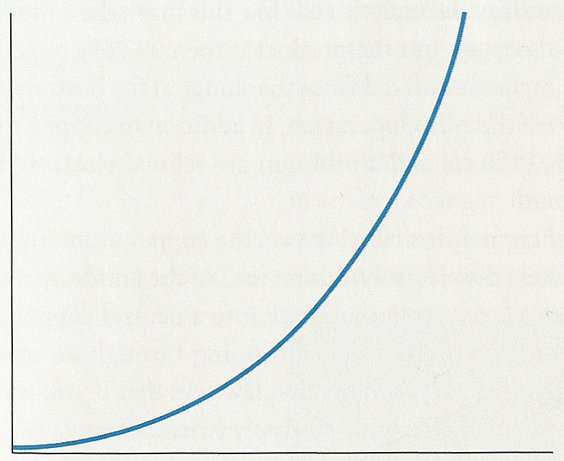
\includegraphics[scale=2.8]{pics/exponential_growth.eps}
\end{center}


\subsection{Granting Privileges requires Trust}
\begin{itemize}
	\item different environments have different trust models
	\item human interactions in small groups strengthen trust
	\item larger groups are divided into smaller, close-nit groups
	\item the more groups you have, the weaker their trust bonds are
\end{itemize}

\subsection{Granting Privileges requires Trust}
\begin{itemize}
	\item different environments have different trust models
	\item human interactions in small groups strengthen trust
	\item larger groups are divided into smaller, close-nit groups
	\item the more groups you have, the weaker their trust bonds are
\end{itemize}
\vspace{.5in}

\begin{center}
	\Huge
	{\bf Trust does not scale.}
	\Normalsize
\end{center}

\subsection{Granting Privileges requires Trust}
\vfill
\begin{center}
	\Huge
	Trust, but (be able to) verify.
	\Normalsize
\end{center}
\vfill

\subsection{Implications of a Multi-User System}
\vspace*{\fill}
\begin{center}
	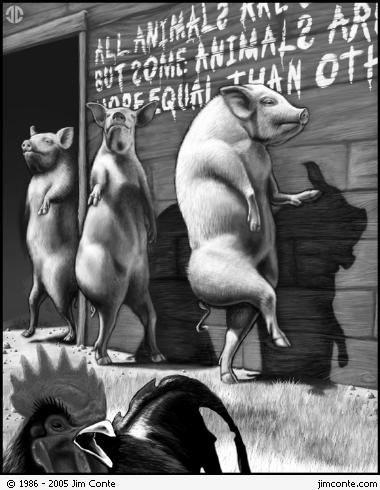
\includegraphics[scale=0.9]{pics/animal_farm.eps}
\end{center}
\vspace*{\fill}

\subsection{Implications of a Multi-User System}
\begin{itemize}
	\item users may want to keep files private
\end{itemize}

\subsection{Implications of a Multi-User System}
\begin{itemize}
	\item users may want to keep files private
	\item users may want to share files
\end{itemize}

\subsection{Implications of a Multi-User System}
\begin{itemize}
	\item users may want to keep files private
	\item users may want to share files
	\item users may (try to gain) access to files they shouldn't have access to
\end{itemize}

\subsection{Implications of a Multi-User System}
\begin{itemize}
	\item users may want to keep files private
	\item users may want to share files
	\item users may (try to gain) access to files they shouldn't have access to
	\item users may (want to) do things that affect other users
\end{itemize}

\subsection{Implications of a Multi-User System}
\begin{itemize}
	\item users may want to keep files private
	\item users may want to share files
	\item users may (try to gain) access to files they shouldn't have access to
	\item users may (want to) do things that affect other users
	\item different users may require different privileges
\end{itemize}

\subsection{Users and User-IDs}
\begin{center}
	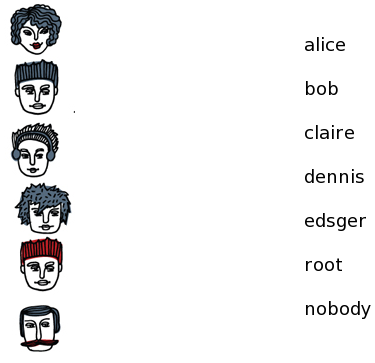
\includegraphics[scale=0.9]{pics/user-sets0.eps} \\
	One-to-one?  Onto?
\end{center}

\subsection{Users and User-IDs}
\begin{center}
	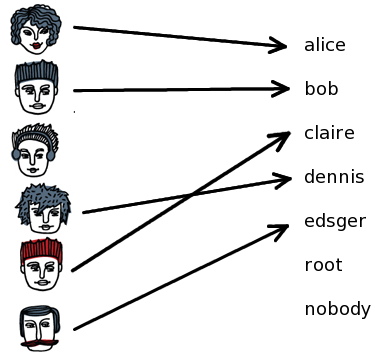
\includegraphics[scale=0.9]{pics/user-sets1.eps} \\
	{\em Not} onto!
\end{center}

\subsection{Users and User-IDs}
\begin{center}
	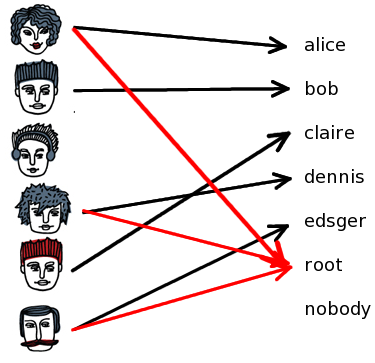
\includegraphics[scale=0.9]{pics/user-sets2.eps} \\
	{\em Not} one-to-one, either!
\end{center}

\subsection{Users and User-IDs}

\begin{center}
	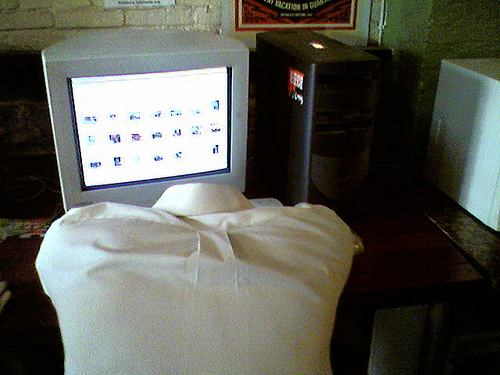
\includegraphics[scale=0.8]{pics/headless.eps} \\
	{\tt nobody}
\end{center}

\subsection{UNIX Fundamentals: User Accounts and File Permissions}
Every account
\begin{itemize}
	\item has a {\em unique} ID
	\item belongs to at least one group
	\item may or may not be password protected
	\item may or may not have a valid login program
\end{itemize}

\subsection{UNIX Fundamentals: User Accounts and File Permissions}
Every account
\begin{itemize}
	\item has a {\em unique} ID
	\item belongs to at least one group
	\item may or may not be password protected
	\item may or may not have a valid login program
\end{itemize}
\addvspace{.5in}
Every file
\begin{itemize}
	\item is associated with a {\em uid} and a {\em gid}
	\item has a number of protection bits
\end{itemize}

\subsection{UNIX Fundamentals: User Accounts and File Permissions}
\vfill
\begin{center}
	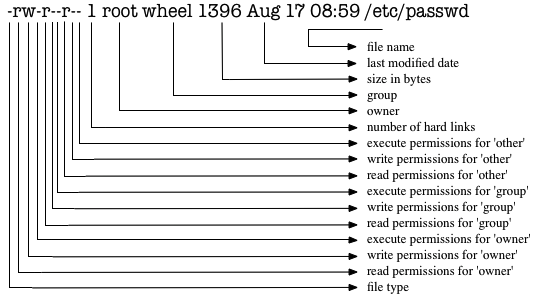
\includegraphics[scale=0.9]{pics/ls-l.eps}
\end{center}
\vfill



\subsection{Unix Groups}
\begin{itemize}
	\item enables {\em arbitrary} collections of users to share resources
	\item information stored in \verb+/etc/group+, format is: \\
		\verb+name:*:GID:user1,user2,...+
	\item most Unix systems impose a limit of 16 or 32 group memberships per
		user
	\item most Unix systems have a common default group for new users (some
		Linux versions deviate)
	\item some Unix systems have group shadow files
\end{itemize}

\subsection{Group Access}
At any but the smallest environments, we find:
\begin{itemize}
	\item a central user database
	\item users divided into different access groups
	\item access to systems is granted primarily by such group membership
	\item privileges on a system are also granted by such group membership
\end{itemize}

\subsection{Group Access}
\begin{center}
	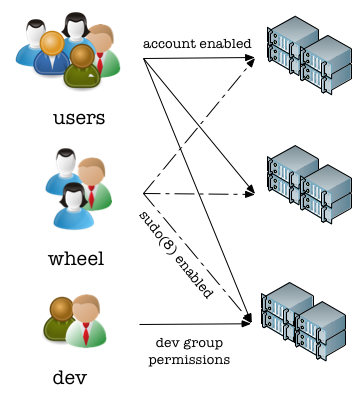
\includegraphics[scale=0.8]{pics/groups-machines.eps}
\end{center}

%\subsection{Adding and Removing Accounts}
%
%\vfill
%In-class exercise: \\
%{\tt https://www.cs.stevens.edu/~jschauma/615/useradd-exercise.html}
%\vfill
%
\subsection{Adding and Removing Accounts}
\vfill
%In-class exercise: \\
%{\tt https://www.cs.stevens.edu/~jschauma/615/useradd-exercise.html} \\
%
%\vspace{.5in}
Accounts management is done centrally; changes are applied to machines via a
configuration management system and/or directory service.
\vfill

\subsection{Ethics}
\begin{center}
	
\includegraphics[scale=2.5]{pics/angel-devil.eps}
\end{center}

\subsection{You are a Super User!}
\begin{center}
	
\includegraphics[scale=1.0]{pics/superman.eps} \\
	\small
	Yes, you are!
	\Normalsize
\end{center}

\subsection{You are a Super User!}
\begin{center}
	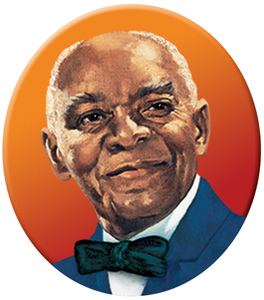
\includegraphics[scale=4.0]{pics/uncle-ben.eps} \\
	\addvspace{.2in}
	\Huge
	``With great power comes great responsibility.''
	\Normalsize
\end{center}


\subsection{Ethics}
The LISA Code of Ethics:
\\

\newcolumntype{S}{>{\centering\arraybackslash} m{.4\linewidth} }
\begin{tabular}{ p{10cm} S }
\begin{itemize}
	\item Professionalism
	\item Personal Integrity
	\item Privacy
	\item Laws and Policies
	\item System Integrity
	\item Education
	\item Social Responsibility
	\item Ethical Responsibility
\end{itemize}
& \multirow{20}{*}{
\includegraphics[scale=1.3]{pics/angel.eps}} \\
\end{tabular}

\subsection{Ethics: This stuff isn't easy!}
\begin{center}
	
\includegraphics[scale=0.3]{pics/snowden.eps}
\end{center}

\subsection{Ethics: Professionalism}
\vfill
\begin{center}
I will maintain professional conduct in the workplace and will not allow
personal feelings or beliefs to cause me to treat people unfairly or
unprofessionally.
\end{center}
\vfill

\subsection{Ethics: Personal Integrity}
\vfill
\begin{center}
I will be honest in my professional dealings and forthcoming about my
competence and the impact of my mistakes. I will seek assistance from
others when required. \\
\vspace{.5in}

I will avoid conflicts of interest and biases whenever possible. When my
advice is sought, if I have a conflict of interest or bias, I will declare
it if appropriate, and recuse myself if necessary.
\end{center}
\vfill


\subsection{Ethics: Privacy}
\vfill
\begin{center}
I will access private information on computer systems only when it is
necessary in the course of my technical duties. I will maintain and
protect the confidentiality of any information to which I may have access,
regardless of the method by which I came into knowledge of it.
\end{center}
\vfill

\subsection{Ethics: Laws and Policies}
\vfill
\begin{center}
I will educate myself and others on relevant laws, regulations, and
policies regarding the performance of my duties.
\end{center}
\vfill

\subsection{Ethics: Communication}
\vfill
\begin{center}
I will communicate with management, users, and colleagues about computer
matters of mutual interest. I will strive to listen to and understand the
needs of all parties.
\end{center}
\vfill

\subsection{Ethics: System Integrity}
\vfill
\begin{center}
I will strive to ensure the necessary integrity, reliability, and
availability of the systems for which I am responsible. \\
\vspace{.5in}

I will design and maintain each system in a manner to support the
purpose of the system to the organization.
\end{center}
\vfill

\subsection{Ethics: Education}
\vfill
\begin{center}
I will continue to update and enhance my technical knowledge and other
work-related skills. I will share my knowledge and experience with others.
\end{center}
\vfill

\subsection{Ethics: Responsibility to the Computing Community}
\vfill
\begin{center}
I will cooperate with the larger computing community to maintain the
integrity of network and computing resources.
\end{center}
\vfill

\subsection{Ethics: Social Responsibility}
\vfill
\begin{center}
As an informed professional, I will encourage the writing and adoption of
relevant policies and laws consistent with these ethical principles.
\end{center}
\vfill

\subsection{Ethics: Ethical Responsibility}
\vfill
\begin{center}
I will strive to build and maintain a safe, healthy, and productive
workplace. \\
\vspace{.5in}

I will do my best to make decisions consistent with the safety, privacy,
and well-being of my community and the public, and to disclose promptly
factors that might pose unexamined risks or dangers. \\
\vspace{.5in}

I will accept and offer honest criticism of technical work as appropriate
and will credit properly the contributions of others. \\
\vspace{.5in}

I will lead by example, maintaining a high ethical standard and degree
of professionalism in the performance of all my duties. I will support
colleagues and co-workers in following this code of ethics.

\end{center}
\vfill

\subsection{At the end of the day...}
\begin{center}
	
\includegraphics[scale=0.5]{pics/thumbsup-borat.eps}
\end{center}

\subsection{Reading}
User Management:
\begin{itemize}
	\item {\em Frisch}: Ch 6; {\em Burgess}: Ch 5;
\end{itemize}
\vspace{.5in}
\begin{itemize}
	\item http://nixsrv.com/llthw/ex23
\end{itemize}
\vspace{.5in}
Ethics:
\begin{itemize}
	\item \verb+https://www.usenix.org/lisa/system-administrators-code-ethics+
	\item \verb+http://www.acm.org/about/code-of-ethics+
\end{itemize}

\subsection{Professional Organizations}
\begin{itemize}
	\item \verb+https://www.usenix.org/+ and \verb+https://www.usenix.org/lisa+
	\item \verb+http://www.lopsa.org/+
	\item \verb+http://www.acm.org/+
	\item \verb+https://www.internetsociety.org/+
	\item \verb+https://www.nanog.org/+
\end{itemize}

\end{document}
